\section{Sintesi e caratterizzazione di \ce{Co(salen)}}
\subsection{Sintesi}
\subsubsection{Procedura sperimentale}
In un pallone da 250 mL, munito di tappo, di rubinetto a due vie e di agitatore magnetico, abbiamo introdotto 2.6 mL  di aldeide salicilica e 100 mL di alcool etilico 95\%, insieme a 0.82 mL  di etilendiammina. Abbiamo avuto pronta precipitazione della base di Schiff di colore giallo. Abbiamo preparato a parte una soluzione di 3.0 g  di \ce{Co(CH3COO)2. 4 H2O} in 30 mL di acqua deionizzata. Questa soluzione è stata posta in imbuto gocciolatore munito di tappo con rubinetto a due vie\footnote{Soluzione di colore rosso rubino}. Dopo quattro cicli di vuoto-azoto, abbiamo gocciolato lentamente (circa 30 minuti) la soluzione del sale di cobalto nel pallone contenente l'immina, mantenuto  sotto azoto a circa 60 °C. Abbiamo lasciato raffreddare a temperatura ambiente e abbiamo filtrato in atmosfera inerte con il filtro a colonna il precipitato, lavando con due porzioni da 20 mL  di acqua deionizzata disaereata ed con 20 mL con alcool etilico disaereato. Abbiamo seccato il solido sotto vuoto controllando dopo un giorno la stabilità del peso in un intervallo di circa un'ora. 
\subsubsection{Apparato sperimentale}
\label{sec:cosalenapp}
La richiesta di un'atmosfera controllata in cui far avvenire la reazione impone l'utilizzo di apparecchiature specifiche. In questo caso il montaggio e la preparazione dell'apparato sono di vitale importanza per la riuscita dell'esperimento. La prima operazione da compiere è quella di preparare il sistema presente sotto la cappa; per fare ciò dovremo compiere alcuni cicli vuoto azoto per essere sicuri che in tutta l'apparecchiatura non sia presente ossigeno. Successivamente si monta la vetreria e si procede a fare alcuni cicli vuoto-azoto anche su di essa. Le valvole e le giunzioni sono state fissate con elastici per garantire l'integrità della struttura. Tutto l'apparato è stato fissato con un morsetto all'intelaiatura metallica presente sotto cappa; per dare maggior supporto al sistema incastreremo sotto il pallone un mantello scaldante grazie all'aiuto di un elevatore.
\begin{figure}[h!]
    \centering
    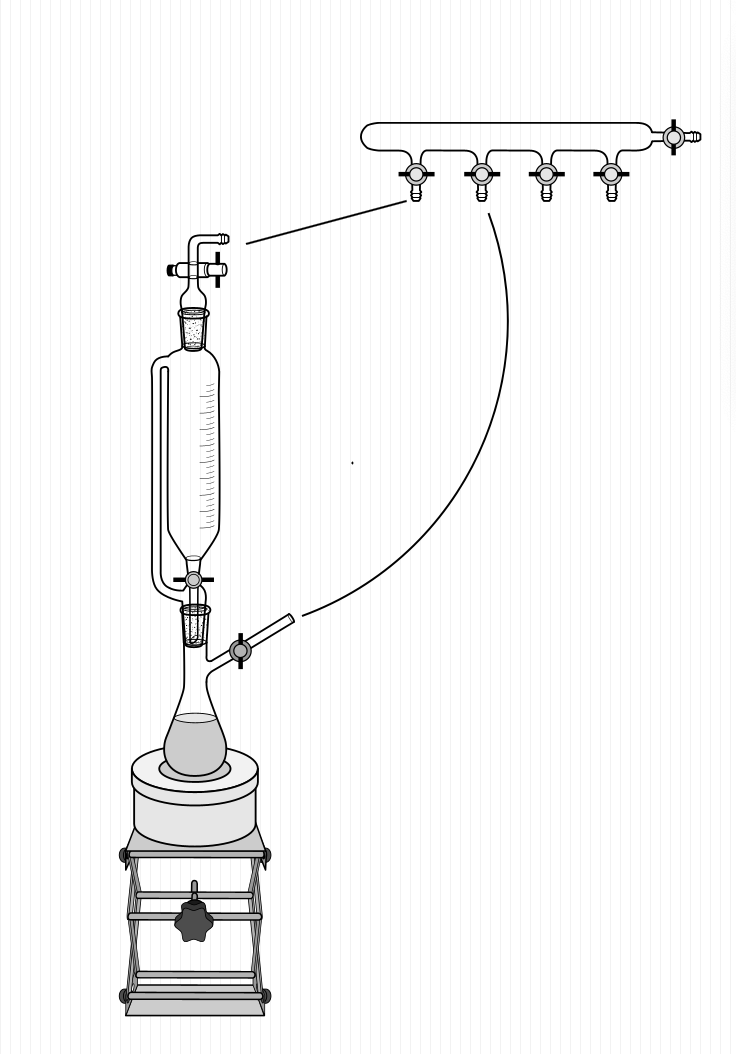
\includegraphics[width=0.4\linewidth]{foto/apparatosalen.png}
    \caption{Schema dell'apparato sperimentale usato per la sintesi. Nello schema mancano le valvole presenti sulle congiunzione tra i tubi e l'apparato. }
    \label{fig:my_label}
\end{figure}
Successivamente alla procedura di sintesi avviene la filtrazione che deve anch'essa essere svolta in atmosfera inerte. Questa fase è di fondamentale importanza per garantire una alta resa di reazione. Abbiamo preparato un filtro a colonna e un adattatore maschio-maschio con coni smerigliati come mostrato in \autoref{fig:filtrosalen}. 
\begin{figure}[ht!]
    \centering
    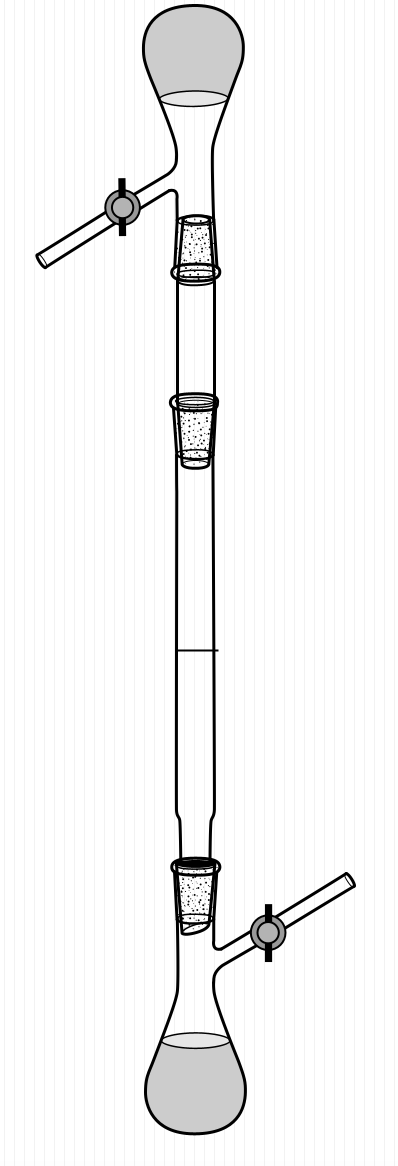
\includegraphics[width=0.15\linewidth]{foto/filtrazione.png}
    \caption{Schema dell'apparato di filtrazione. Di solido le valvole vanno tenute dalla stessa parte.}
    \label{fig:filtrosalen}
\end{figure}


Il pallone sotto va aggiunto successivamente e sarà quello contenente il prodotto da filtrare; prima dobbiamo tappare il sistema con una valvola e fare alcuni cicli di vuoto-azoto per bonificare l'apparato e sotto flusso di azoto collegare il sistema al pallone con il Co(salen)\footnote{Il pallone deve essere scollegato dall'imbuto gocciolatore e collegato al sistema sotto azoto }.


\subsubsection{Commenti e osservazioni}
Dopo l'aggiunta dei reagenti vediamo la formazione dell'immina che si presenterà come solido non molto solubile in etanolo bisogna
scaldare per scioglierla per facilitare la reazione di complessazione.
Bisogna prestare particolare attenzione mentre si maneggia il DMSO perché può passare attraverso la barriera della pelle e portare ciò che vi è disciolto all'interno dell'organismo. Vedi  \autoref{subsec:ossigeno}

Per comprendere i limiti delle misurazioni volumetriche con gli strumenti presenti in laboratorio abbiamo pesato sia la benzaldeide che la etilendiammina. \cite{salenyield}


\subsubsection{Calcoli e analisi dei dati}

In partenza avevamo un numero di moli di reagenti pari a
\[ n_{\ce{Co(OAc)2}}=\frac{3 \mathrm{~g}}{345.58 \mathrm{~g} / \mathrm{mol}}= 12.0 \mathrm{~mmol} \]

\[ n_{\ce{AS}}=\frac{2.6 \mathrm{~mL} \cdot 1.146 \mathrm{~g} / \mathrm{mL} }{30.03 \mathrm{~g} / \mathrm{mol}}=24.6 \mathrm{~mmol} \]
\[ n_{en}=\frac{0.84 \mathrm{~mL} \cdot 0.899 \mathrm{~g} / \mathrm{mL}}{60.10 \mathrm{~g} / \mathrm{mol}}=12.6 \mathrm{~mmol} \]

Considerando quindi la stechiometria $1: 2: 1$ notiamo che il sale è il reagente limitante. 



Calcoliamo la resa 
\[ Y_\% = \frac{n_\text{pro}}{n_{\ce{[Co(en)3]Cl3}}}\cdot 100 \]

Le moli finali sono il rapporto massa della provettà piena di prodotto tolta la tara e la massa molare del prodotto.

\[ n_\text{pro} = \frac{(m_{f} - m_{t})}{M_\text{pro}} 
 = \frac{ 18.8692 \um{g} - 15.1226 \um{g} }{ 325.23 \um{g/mol}} =  \frac{3.7466 \mathrm{~g}}{325.23 \mathrm{~g} / \mathrm{mol}}=11.5 \um{mmol}\]

\[ Y_\% = \frac{n_\text{pro}}{n_{\ce{Co(salen)}}}\cdot 100  = \frac{  11.5 \cdot 10^{-3} \mathrm{~mol}}{12.0 \cdot 10^{-3} \mathrm{~mol}} \cdot 100 =96.0\%\]


\subsection{Spettro IR}


\subsubsection{Preparazione del campione}
Una punta di spatola di campione è stata messa in un mortaio con circa 2 goccie Nujol\textsuperscript{\tiny\textregistered} e pestellata fino a completa omogenizzazione.  Su una finestra di cloruro di sodio viene messa una piccola porzione di miscela, con un'altra finestra si distribuisce e si copre in modo tale da poter essere inserita nell'apposito stand. Si inserisce il tutto nello strumento e si legge lo spettro. Infine, l'apparecchiatura viene smontata, le finestre vengono pulite con iso-propanolo  e lucidate su un panno usando come abrasivo dell'allumina.
\subsubsection{Interpretazione dello spettro}

NaCl assorbe sotto i 1200$\um{cm^{-1}}$, in particolare dallo spettro possiamo notare come sotto i 500$\um{cm^{-1}}$ l'assorbimento è quasi totale ciò dovuto proprio alle finestre di cloruro di sodio che essendo spesse e non trasparenti in quel range di numero d'onda non lasciano passare la radiazione. Nella parte significativa dello spettro, ovvero quella dove l'assorbimento del \ce{NaCl} e del Nujol\textsuperscript{\tiny\textregistered} è ininfluente, possiamo notare le bande tipiche del salen. Lo Nujol\textsuperscript{\tiny\textregistered} essendo una miscela di paraffine a catena corta ha attive all'IR tutte le transizioni relative al C-H che sono molto intense. Possiamo notarle nel intorno destro dei 3000$\um{cm^{-1}}$ e nella zona dei 1400$\um{cm^{-1}}$. Tra le bande del salen le più visibili ci sono gli stretching dei C-H aromatici che si trovano in un intorno sinistro di  3000$\um{cm^{-1}}$, sempre relative alla parte aromatica del salen intorno ai 1800-1900$\um{cm^{-1}}$ troviamo le bande di overtone dell'anello aromatico. Infine, si può notare l'assorbimento relativo allo streatching N=C a circa 1600$\um{cm^{-1}}$.
Il picco di carattere \textit{broad}, oltre 3000$\um{cm^{-1}}$, può essere attribuito alla presenza di acqua o di etilendiammina che entrambi presentano assorbimenti in quella zona con quel tipo di forma. Si può escludere la presenza dell’aldeide salicilica in quanto la regione intorno a 1700$\um{cm^{-1}}$ non presenta assorbimenti.
\begin{figure}[ht!]
    \centering
    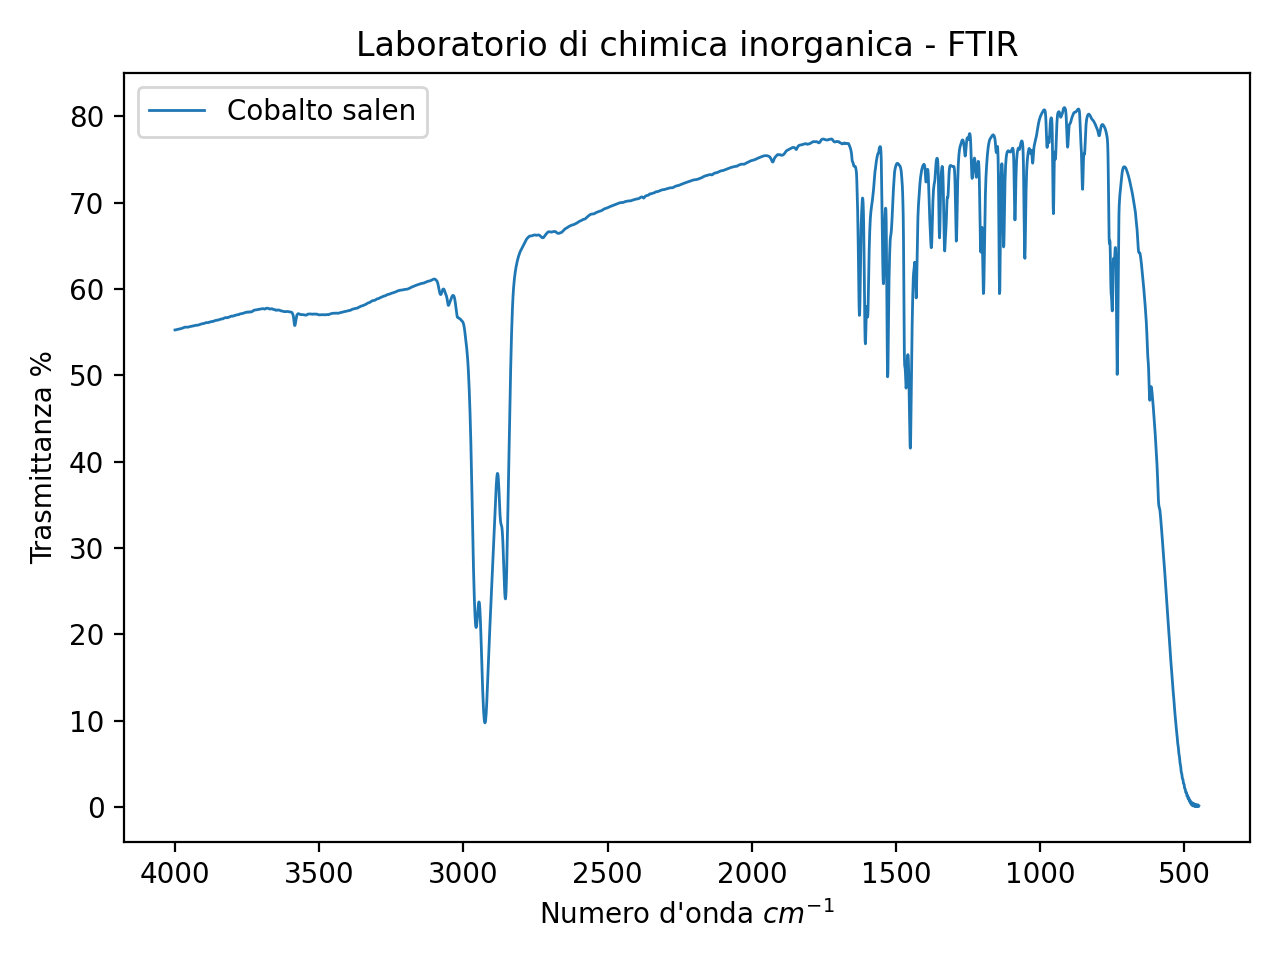
\includegraphics[width=\linewidth]{Relazione/foto/FTIRsalen.png}
    \caption{Spettro FTIR del cobalto salen disperso nel Nujol\textsuperscript{\tiny\textregistered}}
    \label{fig:FTIRsalen}
\end{figure}
\subsection{Assorbimento del diossigeno}\label{subsec:ossigeno}
Abbiamo infine introdotto una piccola quantità di \ce{Co(salen)} finemente polverizzato in un becher e in cui abbiamo anche aggiunto circa 15 mL di DMSO. Abbiamo lasciato sotto agitazione per una notte. Abbiamo notato una variazione di colore della soluzione, la miscela ha perso l'iniziale sfumatura rossiccia diventando di color nero antracite. Abbiamo filtrato sottovuoto la soluzione. Abbiamo aggiunto parte del precipitato presente sul filtro in 10 mL di cloroformio. Abbiamo notato il ritorno del colore rosso segno della deossigenazione del complesso.

